\documentclass[12pt]{article}
\usepackage[margin=1in]{geometry}
\usepackage{amsmath}
\usepackage{graphicx}
\usepackage{stmaryrd}
\usepackage{float}

\author{Kyler Little\vspace{-0.6cm}}
\title{Homework \#3: Machine Learning\vspace{-0.3cm}}
\date{February 26, 2018\vspace{-0.7cm}}

\begin{document}
	\maketitle
	\section*{Problem \#1}
	Suppose that we have three coloured boxes $r$ (red), $b$ (blue), and $g$ (green). Box $r$ contains 3 apples, 4 oranges, and 3 limes; box $b$ contains 1 apple, 1 orange, and 0 limes; and box $g$ contains 3 apples, 3 oranges, and 4 limes. If a box is chosen at random with probabilities $p(r) = 0.2$, $p(b) = 0.2$, $p(g) = 0.6$, and a piece of fruit is removed from the box (with equal probability of selecting any of the items in the box), then what is the probability of selecting an apple? If we observe that the selected fruit is in fact an orange, what is the probability that it came from the green box? \\
	In regards to the first question, we need to compute the marginal probability $p(\text{apple})$. We can do this using the sum and product rules. Let $Y$ denote coloured box.
	\begin{align*}
	p(\text{apple}) &= \sum_{Y}^{} p(\text{apple}, Y) = \sum_{Y}^{} p(\text{apple} \vert Y) p(Y) \\
	&= p(\text{apple} \vert r) p(r) + p(\text{apple} \vert b) p(b) + p(\text{apple} \vert g) p(g)\\
	&= 0.3(0.2) + 0.5(0.2) + 0.3(0.6) \\
	&= 0.34\\
	\end{align*}
	The second question asks us to compute $p(g \vert \text{orange})$. We have all of the conditional properties of the form $P(\text{fruit} \vert \text{box})$, and we want $P(\text{box} \vert \text{fruit})$. This is exactly the purpose of Bayes' Theorem, and so we apply it.
	\begin{align*}
	p(g \vert \text{orange}) &= \frac{p(\text{orange} \vert g) * p(g)}{p(\text{orange})} \\
	&= \frac{p(\text{orange} \vert g) * p(g)}{p(\text{orange} \vert r) p(r) + p(\text{orange} \vert b) p(b) + p(\text{orange} \vert g) p(g)}\\
	&= \frac{0.3(0.6)}{0.4(0.2) + 0.5(0.2) + 0.3(0.6)} \\
	&= 0.5
	\end{align*}
	 
	\section*{Problem \#2}
	Given the following data set containing three attributes and one class, use na\"ive Bayes classifier to determine the class (Yes/No) of Stolen for a Red Domestic SUV.
	\begin{center}
		\begin{tabular*}{280pt}[t]{c |c c c | c}
			Example No. & Color & Type & Origin & Stolen? \\
			\hline \hline
			1 & Red & Sports & Domestic & Yes \\
			2 & Red & Sports & Domestic & No \\
			3 & Red & Sports & Domestic & Yes \\
			4 & Yellow & Sports & Domestic & No \\
			5 & Yellow & Sports & Imported & Yes \\
			6 & Yellow & SUV & Imported & No \\
			7 & Yellow & SUV & Imported & Yes \\
			8 & Yellow & SUV & Domestic & No \\
			9 & Red & SUV & Imported & No \\
			10 & Red & Sports & Imported & Yes \\
		\end{tabular*}
	\end{center}
	Let $x^* = [\text{Red} \ \text{SUV} \ \text{Domestic}]^T$. To use na\"ive Bayes' classifier, we shall calculate $P(\text{Yes} \, \vert \, x^*)$ and $P(\text{No} \, \vert \, x^*)$. Whichever is larger will be the decision. To start, we will calculate $P(\text{Yes} \, \vert \, x^*)$. We ignore the denominators because they are the same, and we only care which is larger.
	\begin{align*}
	P(\text{Yes} \, \vert \, x^*) &\propto P(x^* \, \vert \, \text{Yes}) * P(\text{Yes}) \\
	&\propto (P(\text{Red} \, \vert \, \text{Yes}) * P(\text{SUV} \, \vert \, \text{Yes}) * P(\text{Domestic} \, \vert \, \text{Yes})) * P(\text{Yes}) \\
	&\propto ((3/5)*(1/5)*(2/5))*0.5\\
	&\propto 0.024 \\
	\end{align*}
	Next, we calculate $P(\text{No} \, \vert \, x^*)$, again ignoring the denominator.
	\begin{align*}
	P(\text{No} \, \vert \, x^*) &\propto P(x^* \, \vert \, \text{No}) * P(\text{No}) \\
	&\propto (P(\text{Red} \, \vert \, \text{No}) * P(\text{SUV} \, \vert \, \text{No}) * P(\text{Domestic} \, \vert \, \text{No})) * P(\text{No}) \\
	&\propto ((2/5)*(3/5)*(3/5))*0.5\\
	&\propto 0.072 \\
	\end{align*}
	Since $P(\text{No} \, \vert \, x^*) > P(\text{Yes} \, \vert \, x^*)$, our decision is  ``No.''
	
	
	\section*{Problem \#3}
	This question is about na\"ive Bayes classifier. Please do the following: \\
	(a) State what is the simplifying assumption made by na\"ive Bayes classifier. \\
	The simplifying assumption is that each $x_i$ of the input vector are conditionally independent, given the target value (classification). In other words, the probability of observing $x_{1}, x_{2}, ..., x_{d}$, given the target value, is just the product of the probabilities of the individual attributes: $P(x_{1}, x_{2}, ..., x_{d} \, \vert \, y) = \prod_{i=1}^{d}P(x_{i} \, \vert \, y)$. \\
	(b) Given a binary-class  classification  problem  in  which the  class  labels  are  binary,  the  dimension  of feature is $d$, and each attribute can take $k$ different values. Please provide the numbers of parameters to  be  estimated  with  AND  without  the  simplifying  assumption. Briefly  justify  why the  simplifying assumption is necessary. \\
	\paragraph{}
	Without the simplifying assumption, one has to enumerate all possible values of the input space, and for each distinct value, calculate its frequency in the training data to obtain an estimate. The problem with this is that the number of these parameters needed to be estimated is the number of target values (i.e. class labels) times the number of distinct values in the input space minus one (the last value need not be estimated since it is one subtract the sum of the others). This is a very large number of parameters to be estimated. For instance, in our situation, each $x_i$ can take $k$ different values, and there are $d$ attributes. By the multiplication rule for combinatorics, there are $k * k * \cdots * k = k^d$ distinct values of the input space. The last value need not be estimated; in fact, it is not free to vary. Thus, the number of degrees of freedom is $k^{d} - 1$. Since we must estimate this number of parameters for each class or target value, there are $2(k^{d} - 1)$ parameters to be estimated. \par
	On the other hand, when the simplifying assumption is made, we are able to estimate far less parameters. We need only estimate the number of target values (i.e. class labels) times the number of distinct attributes-- $2d$ in this case. \par
	Besides the fact that this simplifying assumption significantly reduces the number of parameters to be estimated ($2(k^{d} - 1) \ll 2d$, in general), the assumption is necessary for other reasons as well. Without the assumption, the model wouldn't generalize well to unseen data. For instance, if the model hadn't seen a particular input vector in its training data, there wouldn't be a prediction at all, since $P(x \, \vert \, y_{1}) = P(x \, \vert \, y_{2})= 0$. Thus, an extremely large training data set would be needed in order for the model to function correctly. The size of the training data set $N$ would need to be much larger than $k^{d}$, which is very infeasible in reality. 
	
	\section*{Problem \#4}
	Assume we want to classify science texts into three categories— physics, biology and chemistry. The  following  probabilities  have  been  estimated  from  analyzing  a  corpus  of  pre-classified  web-pages gathered from Yahoo.
		\begin{center}
			\begin{tabular*}{245pt}[t]{l | c c c}
				c & Physics & Biology & Chemistry \\
				\hline
				P(c) & 0.35 & 0.40 & 0.25  \\
				P(atom $\vert$ c) & 0.1 & 0.01 & 0.2 \\
				P(carbon $\vert$ c) & 0.005 & 0.03 & 0.05 \\
				P(proton $\vert$ c) & 0.05 & 0.001 & 0.05  \\
				P(life $\vert$ c) & 0.001 & 0.1 & 0.008 \\
				P(earth $\vert$ c) & 0.005 & 0.006 & 0.003  \\
			\end{tabular*}
		\end{center}
	Assuming that the probability of each evidence word is independent of other word occurrences given the category of the text, compute the (posterior) probability for each of the possible categories each of the following short texts; and based on that, their most likely classification. Assume that the categories are disjoint and exhaustive (i.e., every text is either physics, or biology or chemistry, and no text can be more than one). Assume that words are first stemmed to reduce them to their base form (atoms $\rightarrow$ atom) and ignore any words that are not in the table:
	\begin{center}
	\begin{tabular*}{250pt}[t]{l}
	A: the carbon atom is the foundation of life on earth \\
	B: the carbon atom contains 12 protons. \\
	\end{tabular*}
	\end{center}
	This is a job for na\"ive Bayes' classifier. The first task will be to vectorize A and B. We will use a binary vector, where words `atom', `carbon', `proton', `life', and `earth' correspond to entries one through five of the vector. If the word appears at least once, then the entry will be set to 1. Otherwise, it will be 0.
	\begin{center}
		\begin{tabular*}{250pt}[t]{l}
			A = $[1 \ 1 \ 0 \ 1 \ 1]^T$ \\
			B = $[1 \ 1 \ 1 \ 0 \ 0]^T$ \\
		\end{tabular*}
	\end{center}
	The decision will be:
	\begin{equation*}
	\text{arg max}_{v} \prod_{j=1}^{5} p_{j}(x^{j} \, \vert \, y=v) p(y = v)
	\end{equation*}
	where $v \in \lbrace {\text{Physics}, \text{Biology}, \text{Chemistry}}\rbrace$. We begin with classifying A.
	\begin{align*}
	\hat{y} &= \text{arg max}_{v} \prod_{j=1}^{5} p_{j}(x^{j} \, \vert \, y=v) p(y = v) \\
	&= \text{arg max} ( \prod_{j=1}^{5} p_{j}(x^{j} \, \vert \, y=\text{Physics}) p(y = \text{Physics}), \\
	& \qquad\qquad\quad \prod_{j=1}^{5} p_{j}(x^{j} \, \vert \, y=\text{Biology}) p(y = \text{Biology}), \\
	& \qquad \qquad \quad \prod_{j=1}^{5} p_{j}(x^{j} \, \vert \, y=\text{Chemistry}) p(y = \text{Chemistry}) ) \\
	&= \text{arg max} ((0.1*0.005*0.95*0.001*0.005)*0.35,\\
	&\qquad\qquad\quad (0.01*0.03*0.999*0.1*0.006)*0.40,\\
	&\qquad\qquad\quad (0.2*0.05*0.95*0.008*0.003)*0.25) \\
	&= \text{arg max} (8.3125 \cdot 10^{-10}, 7.1928 \cdot 10^{-8},5.7000 \cdot 10^{-8}) \\
	&= \text{arg } 7.1928 \cdot 10^{-8} \\
	&= \text{Biology} \\
	\end{align*}
	Next, we classify B.
	\begin{align*}
	\hat{y} &= \text{arg max}_{v} \prod_{j=1}^{5} p_{j}(x^{j} \, \vert \, y=v) p(y = v) \\
	&= \text{arg max} ( \prod_{j=1}^{5} p_{j}(x^{j} \, \vert \, y=\text{Physics}) p(y = \text{Physics}), \\
	& \qquad\qquad\quad \prod_{j=1}^{5} p_{j}(x^{j} \, \vert \, y=\text{Biology}) p(y = \text{Biology}), \\
	& \qquad \qquad \quad \prod_{j=1}^{5} p_{j}(x^{j} \, \vert \, y=\text{Chemistry}) p(y = \text{Chemistry}) ) \\
	&= \text{arg max} ((0.1*0.005*0.05*0.999*0.995) * 0.35,\\
	&\qquad\qquad\quad (0.01*0.03*0.001*0.9*0.994)*0.40,\\
	&\qquad\qquad\quad (0.2*0.05*0.05*0.992*0.997)*0.25) \\
	&= \text{arg max} (8.6975 \cdot 10^{-6}, 1.0735 \cdot 10^{-7}, 1.2363 \cdot 10^{-4}) \\
	&= \text{arg } 1.2363 \cdot 10^{-4} \\
	&= \text{Chemistry} \\
	\end{align*}
	
	\section*{Problem \#5}
	Consider the following table of observations:
	\begin{center}
		\begin{tabular*}{340pt}[t]{c | c c c c | c}
			No. & Outlook & Temperature & Humidity & Windy & Play Golf? \\
			\hline \hline
			1 & sunny & hot & high & false & N \\
			2 & sunny & hot & high & true & N \\
			3 & overcast & hot & high & false & Y \\
			4 & rain & mild & high & false & Y \\
			5 & rain & cool & normal & false & Y \\
			6 & rain & cool & normal & true & N \\
			7 & overcast & cool & normal & true & Y \\
			8 & sunny & mild & high & false & N \\
			9 & sunny & cool & normal & false & Y \\
			10 & rain & mild & normal & false & Y \\
			11 & sunny & mild & normal & true & Y \\
			12 & overcast & mild & high & true & Y \\
			13 & overcast & hot & normal & false & Y \\
			14 & rain & mild & high & true & N \\
		\end{tabular*}
	\end{center}
	From the classified examples in the above table, construct two decision trees (by hand) for the classification "Play Golf." For the  first tree, use Temperature as the root node. (This  is
	a really bad  choice.) Continue the construction  of  tree  as  discussed  in  class  for  the  subsequent  nodes using information  gain. Remember  that different attributes can be used in different branches on a given level of the tree. For the second tree, follow the  Decision Tree Learning  algorithm described  in class. At  each step,  choose  the  attribute  with  the  highest information gain. Work out the computations of information gain by hand and draw the decision tree.
	\paragraph{}
	For the first tree, we use Temperature as the root node. As we shall see in construction of the second tree, Temperature is the worst of the four choices. Without considering the IG of the decision, we propagate examples into their respective branches. Four go to the `hot' branch; six go to the `mild' branch; four go to the `cool' branch. \par
	Before diving into the messier branches, I will first finish the `hot' branch. If we choose ``Outlook" as the next attribute to classify by, the IG is maximized. Two examples go to the `sunny' branch (both `N'), while the other two examples go to the `overcast' branch (both `Y'). No examples are propagated to the `rain' branch, so its decision is based on the majority rule at the parent node (``Outlook" in this case). Since the split is even, we go to the next parent node up: ``Temperature." Its decision is `Y' since those account for the majority of examples. \par
	Next, we will finish the `mild` branch stemming from the root node. The best choice is Outlook ($\text{IG}_{\text{Outlook}} = 0.126 > \text{IG}_{\text{Humidity}} = \text{IG}_{\text{Windy}} = -0.082$). Next, we note that only one instance was propagated to the `overcast' branch, so it becomes a leaf node with decision `Y'. Continuing down the `sunny' branch, we note that the ``Humidity" attribute maximizes the IG (i.e. all propagated instances belong to one class), resulting in the `normal' branch leading to a `Y' leaf node and the `high' branch leading to a `N' leaf node. Lastly, we continue down the `mild'--`rain' branch. From here, it's easy to see that the ``Windy" attribute fully segregates the classes, maximizing its IG. The `true' branch leads to a `N' leaf node, while `false' leads to a `Y' leaf node. \par
	Finally, we finish the tree by completing the `cool' branch stemming from the root node. The best attribute choice is either ``Windy" or ``Outlook" since they have identical IGs ($\text{IG}_{\text{Outlook}} = \text{IG}_{\text{Windy}} = 0.3113 > \text{IG}_{\text{Humidity}} = 0$). We will pick ``Windy" since the result is essentially the same either way. The `false' branch leads to a `Y' leaf node, while the `true' branch leads to our last two examples (one `Y' and one `N'). From here (node located at `cool'--`true'), we select ``Outlook" as our final attribute choice since it maximizes IG. One instance is propagated to the `rain' branch (resulting in a `N' leaf node), while the other is propagated to the `overcast' branch (resulting in a `Y` leaf node). The `sunny' branch is determined by majority vote from the parent node. As before, it is undecided, so we go to the next parent node up: ``Temperature." Its decision is again `Y' since those account for the majority of examples. \par
	Finally, we construct the tree.
	\begin{figure}[H]
		\begin{center}
			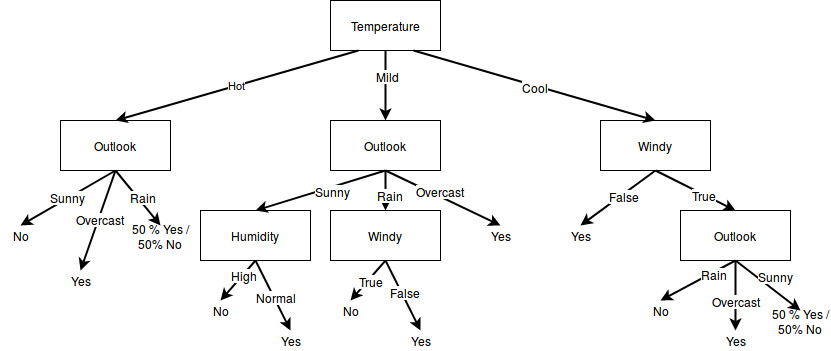
\includegraphics[width=440pt]{hw3_ml_tree1.jpg}
			\caption{Decision Tree (bad)}
			\label{fig:tree1}
		\end{center}
	\end{figure}
	For construction of the second tree, we follow the Decision Tree Learning Algorithm. For any given node, we pick the attribute with the largest information gain (IG). If $I$ is the entropy function, then we always select the attribute $v$ such that:
	\begin{equation*}
	\text{Selected Attribute} = \text{max arg}_{v} \ \text{IG} = \text{max arg}_{v} \ (I_{\text{before}}-I_{\text{after}})
	\end{equation*}
	Note that $I_{\text{after}}$ is dependent upon $v$. Starting from the root node, we compute the selected attribute. The $IG$ is computed in the following order: Outlook, Temperature, Humidity, Windy.
	\begin{align*}
	\text{Selected Attribute} &= \text{max arg}_{v} \  (1-(\frac{5}{14}I(\frac{3}{5},\frac{2}{5}) + \frac{4}{14}I(\frac{0}{4},\frac{4}{4}) + \frac{5}{14}I(\frac{2}{5},\frac{3}{5})), \\
	&\qquad\qquad\qquad 1-(\frac{4}{14}I(\frac{1}{2},\frac{1}{2}) + \frac{6}{14}I(\frac{2}{6},\frac{4}{6}) + \frac{4}{14}I(\frac{1}{4},\frac{3}{4})), \\
	&\qquad\qquad\qquad 1-(\frac{7}{14}I(\frac{3}{7},\frac{4}{7}) + \frac{7}{14}I(\frac{1}{7},\frac{6}{7})), \\
	&\qquad\qquad\qquad 1-(\frac{6}{14}I(\frac{3}{6},\frac{3}{6}) + \frac{8}{14}I(\frac{2}{8},\frac{6}{8}))) \\
	&= \text{max arg}_{v} \ (0.3065, 0.0889, 0.2117, 0.1078) \\
	&= \text{Outlook}
	\end{align*}
	As we can see, the root node will be ``Outlook." In this case, we see that if the Outlook is `overcast', the decision is always `Y.' Thus, we obtain a leaf node there. For the other two branches-- sunny and rain--, it's easy to see that maximum information gain can be obtained by using the ``Humidity" attribute on the `sunny' branch and the ``Windy" attribute on the `rain' branch. Because the information gain is maximized (i.e. all propagated instances belong to one class), there is no need to check other potential attributes. We instantly have leaf nodes. The resulting tree is below.
	\begin{figure}[H]
		\begin{center}
			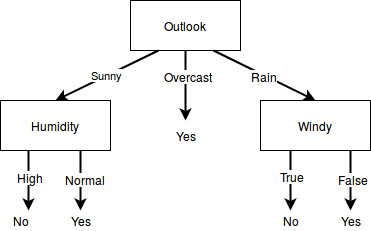
\includegraphics[width=300pt]{hw3_ml_tree2.jpg}
			\caption{Decision Tree (correct)}
			\label{fig:tree2}
		\end{center}
	\end{figure}
	Note: all figures were drawn on ``draw.io."
	
\end{document}